%
% File naacl2019.tex
%
%% Based on the style files for ACL 2018 and NAACL 2018, which were
%% Based on the style files for ACL-2015, with some improvements
%%  taken from the NAACL-2016 style
%% Based on the style files for ACL-2014, which were, in turn,
%% based on ACL-2013, ACL-2012, ACL-2011, ACL-2010, ACL-IJCNLP-2009,
%% EACL-2009, IJCNLP-2008...
%% Based on the style files for EACL 2006 by 
%%e.agirre@ehu.es or Sergi.Balari@uab.es
%% and that of ACL 08 by Joakim Nivre and Noah Smith

\documentclass[11pt,a4paper]{article}
\usepackage[hyperref]{naaclhlt2019}
\usepackage{times}
\usepackage{latexsym}

\usepackage{url}

%\aclfinalcopy % Uncomment this line for the final submission
%\def\aclpaperid{***} %  Enter the acl Paper ID here

%\setlength\titlebox{5cm}
% You can expand the titlebox if you need extra space
% to show all the authors. Please do not make the titlebox
% smaller than 5cm (the original size); we will check this
% in the camera-ready version and ask you to change it back.

\newcommand\BibTeX{B{\sc ib}\TeX}

%%%%%neww added commands by writer%%%%%%
\newcommand{\PA}[1]{{\textcolor{blue}{#1}}}
\newcommand{\question}[1]{{\textcolor{orange}{#1}}}

\renewcommand{\labelitemii}{$\diamond$}

\usepackage{amssymb}
\usepackage{amsmath}
\usepackage{amsfonts}
\usepackage{graphicx}
\usepackage[ruled,linesnumbered]{algorithm2e}

%%%%%neww added commands by writer%%%%%%

%\title{A Navigation Web Search System for  Expert Tracking \\ Using Deep Reinforcement Learning}
\title{Deep Reinforcement Learning for Expert Mobility Tracking from Web Search Results}

\author{Pegah Alizadeh \\
  Affiliation / Address line 1 \\
  Affiliation / Address line 2 \\
  Affiliation / Address line 3 \\
  {\tt email@domain} \\\And
  Josue Urbina \\
  Affiliation / Address line 1 \\
  Affiliation / Address line 2 \\
  Affiliation / Address line 3 \\
  {\tt email@domain}
  Carl Posthuma \\
  Affiliation / Address line 1 \\
  Affiliation / Address line 2 \\
  Affiliation / Address line 3 \\
  {\tt email@domain} 
  Jorge Garcia \\
  Affiliation / Address line 1 \\
  Affiliation / Address line 2 \\
  Affiliation / Address line 3 \\
  {\tt email@domain} 
  Ivan Meza \\
  Affiliation / Address line 1 \\
  Affiliation / Address line 2 \\
  Affiliation / Address line 3 \\
  {\tt email@domain} 
  Luis Pineda \\
  Affiliation / Address line 1 \\
  Affiliation / Address line 2 \\
  Affiliation / Address line 3 \\
  {\tt email@domain}
  \\}
\date{}

\begin{document}
\maketitle
\begin{abstract}

  This paper presents an original approach for extracting experts mobility traces from the web based on deep reinforcement learning. In the broad context of Digital Humanities, the goal of our work is to assist migration sociologists studying expert's international mobility trajectories with natural language processing methods. Deep-Q networks have recently shown promising results improving information extraction methods from web results. Given an expert's name, our method harvests information from web search engines and extracts the optimal expert's mobility trajectory (a set of triplets containing institution, city and year) from it by means of a Deep-Q network and various neural network architectures for the Q-value function approximation. This paper presents experimental evidence improving the current state of the art on expert finding, and extending the existing task with a chronological graph of the experts professional trajectory. 

  %We present at a first time, a people tracking system (specifically the expert people with available and extractable information in the web) as an application of deep reinforcement learning and natural language processing methods to the immigration sociology. The Deep Q-network has been used for extracting information from huge size text datasets and finding the most precise name entities. In this paper, for the sociology term of usage, we propose a method for tracking a give person name and extracting her optimal professional trajectory by exploring the web and generating as less as possible number of queries. Our proposed approach is based on a Deep Q-network method with various neural networks for the Q-value function approximation. We improve the existed people search systems by tracking the experts professional trajectories instead of just labeling them as a mobile or local person w.r.t their origin countries.  
\end{abstract}

\section{Introduction}
Luis Fernandez left his origin country (Argentina) in  $2005$ for doing a PHD in telecommunication. What does he do now? where is he now? where were other universities or organisations that he has worked for so far? for which periods? what are his specialties? In the other words what is his \textit{professional track}. Sociologists of immigration and particularly those who are interested in ``brain drain" domain requires great deal of time, manual internet search or data source search (such as CVs, personal Web Pages, etc.) to answer such fine-grained examples \cite{Auriol2010,Meyer2006}.

%%%%%%%%%%%
\begin{figure}[!t]
\centering
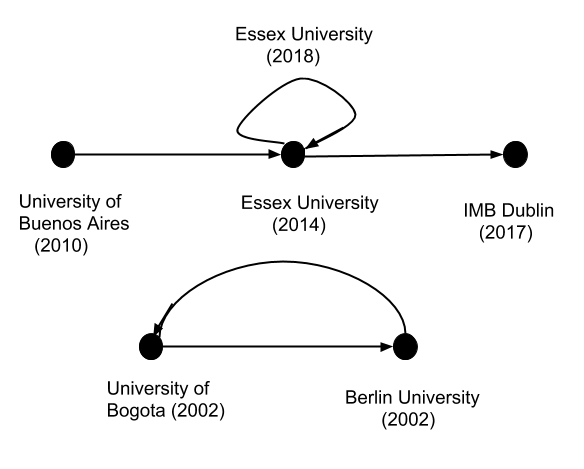
\includegraphics[scale=0.3]{./images/trajectory.png}
\caption{The graph in the top demonstrates Luis Fernandez's trajectory while the bottom one shows a local expert trajectory. }
\label{fig:traj}
\end{figure}
%%%%%%%%%

\PA{may be some state of the art should be added through the following explanation}\\
In this work, we are interested in extracting a trajectory for each given expert including her organisation names and the related years by searching their given names through the web and extracting as accurate as possible name entities (In the rest of this work, by the name entities we mean the organisation names, university names or dates) from the web.  For instance, a researcher as ``Luis Fernandez" has a mobile professional trajectory with various oraganisations and year of experience as figure~\ref{fig:traj} (top graph) though another person (the bottom graph) has a local professional trajectory and he works in his original country recently.  

An intuitive approach for tracking an expert professional trajectory contains two parts: querying various search engines with different keywords and extracting name entities from the list of snippets generated by each query. Here the main dilemma is that when is the proper moment for generating a new query and which snippets should be taken into account for extracting more accurate name entities w.r.t the expert professional trajectory. %According to figure~\ref{fig:navigate} 

In this paper, we propose a method for tracking each given expert's profession using deep reinforcement learning (DRL) approach. Deep Q-network (DQN) usage in various problems and the tracking issue as a planning problem motivate us concentrating on this approach. Some recent problems have been solved by using Deep Q-network method such as information extraction \citep{narasimhan2016improving}, object detection in images \cite{Caicedo2015}, solving arithmetic word problems \cite{wang2018} and text generation \citep{Guo2015}. Inspiring Narasimhan et al. \shortcite{narasimhan2016improving} work on the information extraction problem for huge size search spaces and regarding tracking expert problem as a optimal policy search in RL, we consider deep Q-network and various neural network models to learn Q-value functions and approximate the optimal expert's track for a given expert name.  

Our main contributions in this paper are as the following:
\begin{itemize}
\item To the best of our knowledge, a people tracking system based on Deep RL methods is first presented in this paper.
\item The Q-value function depends on the sequence of snippets selection through the web. For this reason, we replace the neural network of Deep Q-network \cite{mnih2015} with a long Short Term Memory (LSTM) network and \PA{improves the result by \%  }
\item \PA{We test our methods on .... dataset and improve the results by .... }
\end{itemize}

%\begin{figure}[!t]
%\centering
%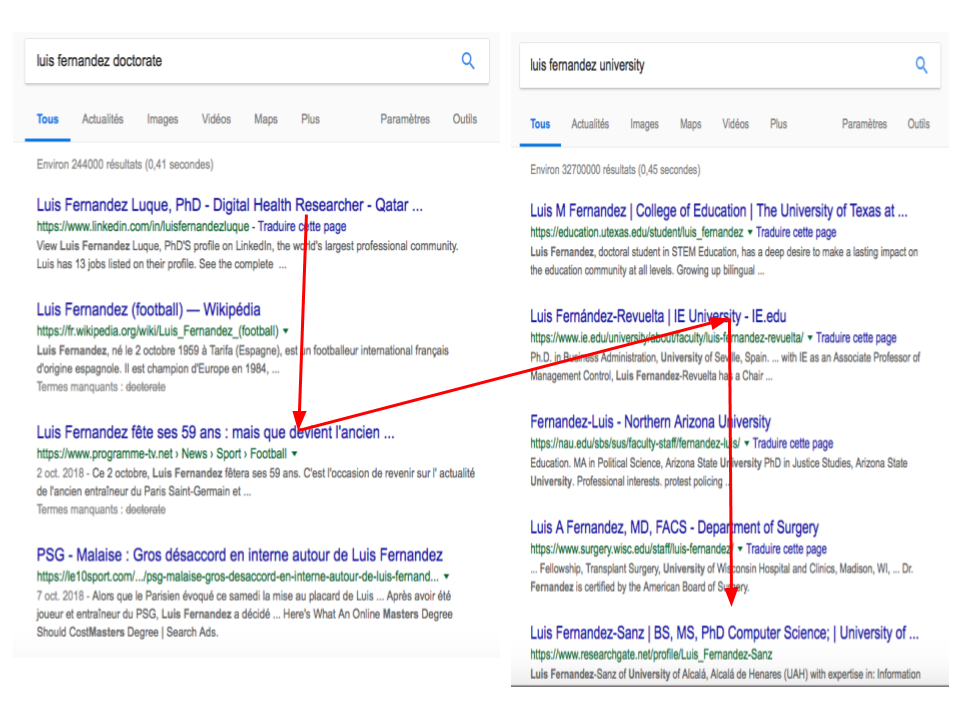
\includegraphics[scale=0.22]{./images/navigate.png}
%\caption{\PA{This figure motivates the usage of reinforcement learning in navigating web. But it has two problems: quality and confidential names. Even if I selected a common general Spanish name.}}
%\label{fig:navigate}
%\end{figure}



\section{Related Work}

In this section we review the literature of the \textit{Deep Reinforcement Learning (DRL)} methods used for the web based information extraction problems. We also introduce a background on the application of \textit{Natural Language Processing (NLP)} and DRL methods on sociology of migration application and Web People Search (WPS) tasks. 

\paragraph{Web People Search (\PA{or any similar title reviewing the literature for navigating immigration data base in the web})}

\paragraph{Deep Reinforcement Learning}
In the Reinforcement Learning (RL) environment with a state set $S = s_1, \cdots, s_m$ and a  set of possible actions $A = a_1, \cdots, a_m$, the agent interacts with the environment by selecting an action $a$ in each state $s$ and going to the next state $s'$ until the terminal state condition is satisfied. This process is guided by a function namely \textit{policy} $\pi : S \longrightarrow A$ by interacting the environment. The policy is calculable by assigning a punishment or reward $r(s, a)$ to each selected action $a$ in any state $s$ and maximizing the expected some of rewards \cite{sutton1998}.  

A way of defining the quality of policies is the Q-value function $Q : S \times A \longrightarrow \mathbb{R}$ given by: 
$$Q^{\pi}(s, a) = \mathbb{E}[R_1+ \gamma R_2 + \cdots | s_0 = s, a_0 =a, \pi]$$

which is the expectation of sum of rewards by starting in state $s$ taking action $a$ and following policy $\pi$. Here $\gamma \in (0, 1]$ is a discount factor for future rewards. Considering the Q-value of the \textit{optimal policy} as $Q^*$, then the optimal policy is: $\pi^*(s) = \text{argmax}_a Q^{\pi^*}(s, a) \; \forall  s \in S$.  

Q-learning algorithm \cite{sutton1998} is a model free method for learning the optimal Q-value function. Since Q-value function should be calculated for each sequence of state/actions, computing $Q(s, a)$ for real environments with great number of (or continuous) states or actions  is impractical.  To tackle this problem Mnih et al. \shortcite{mnih2015} introduce the Deep Q-network algorithm for approximating the Q-value function with a non-linear multi layer convolutional neural network.  Given state $s$ and action $a$, the DQN gives $Q(s, a; \theta)$ value where $\theta$ are parameters for the neural network. (\question{If we model the Q-value function as $Q(s, .; \theta)$ where gets sate $s$ and outputs a vector of action values is better in term of calculation time. Our current model is the naive form.})




\section{Framework and Solution}
Using a similar framework as Narasimhan et al. \shortcite{narasimhan2016improving}, we model our web navigator model as a Markov Decision Process (MDP) \cite{puterman1994}. . .

This MDP is defined as a tuple $M(S, A, P, r, \gamma)$ where $S$ is a set of states, $A$ is a set of actions, $P :S\times A  \times S  \longrightarrow [0,1]$ is a transition function where $P(s'|s,a)$ encodes the probability of going to state $s'$ by being in state $s$, and choosing action $a$; $r : S \times A \longrightarrow R$ is a reward function (or penalty, if negative) obtained by choosing action $a$ in state $s$. Each 

blah blah blah

\section{Data}
We test the experiments on (\PA{three?}) different datasets.  The first dataset is a collected dataset including (\PA{how many persons in experiment?})  researchers and experts from central and sound America. A few information such as year, organisation, graduate degree, original country, domain and destination country of each person who left his/her original country for, is supported in the dataset prepared by the sociologists. 

Another dataset is \PA{Jorge dataset?}

Finally we experiment the navigation web system on \PA{shooting dataset with LSTM instead of NN in DQN}

\section{Experiments}

\section{Conclusions}

\section*{Acknowledgments}

\bibliography{naaclhlt2019}
\bibliographystyle{acl_natbib}

\appendix

\section{Appendices}
\label{sec:appendix}


\section{Supplemental Material}
\label{sec:supplemental}

\end{document}
